\documentclass[research]{BMSTU-IU8}

\usepackage{todonotes}
\usepackage{lipsum}
\SetLipsumText{fishes}

\student{Железцов Н.В.}
\theme{Анализ и формальная верификация алгоритма консенсуса Raft}
\group{ИУ8-94}

\supervisor{Колесников А.В.}

% \theme{Тест \hfill} % Тема для НИРСа заполняется по-другому
\studentFullName{Железцов Никита Владимирович}
\profile{20У474}
\speciality{10.05.01 <<Компьютерная безопасность>>}
\specialization{10.05.01\_01 <<Математические методы защиты информации>>}

\newacronym{bd}{БД}{База данных.}
\newacronym{subd}{СУБД}{Система управления базами данных.}
\newacronym{cdc}{CDC}{Change Data Capture.}
\newacronym{gc}{GC}{Change Data Capture.}
\newacronym{ddl}{DDL}{Data Definition Language.}
\newacronym{dql}{DQL}{Data Query Language.}
\newacronym{dml}{DML}{Data Manipulation Language.}
\newacronym{dcl}{DCL}{Data Control Language.}
\newacronym{wal}{WAL}{Write-ahead log.}
\newacronym{lsn}{LSN}{Log sequence number.}
\newacronym{uri}{URI}{Uniform resource identifier.}
\newacronym{id}{ID}{Identifier.}
\newacronym{uuid}{UUID}{Universally unique identifier.}
\newacronym{ro}{RO}{Read-only.}
\newacronym{rw}{RW}{Read-write.}


\newglossaryentry{id7}{
    name={Анонимная реплика},
    description={это тип реплики, которая подключается к ведущему узлу для получения данных, но не участвует в кворуме репликации и не может стать мастером репликасета.}
}

\newglossaryentry{id1}{
    name={База данных (БД)},
    description={это организованная коллекция данных, которая структурирована таким образом, чтобы данные можно было легко хранить, управлять, изменять и извлекать.},
}

\newglossaryentry{id3}{
    name={Захват изменения данных (Change Data Capture, CDC)},
    description={это программное обеспечение для отслеживания и записи изменений, происходящих в данных базы данных. Оно позволяет фиксировать все вставки, обновления и удаления записей в режиме реального времени или с минимальной задержкой, что позволяет синхронизировать данные между различными системами, вести аудит изменений, и создавать системы резервного копирования или аналитики.}
}

\newglossaryentry{id6}{
    name={Кластер},
    description={это совокупность нескольких репликасетов, каждый из которых чаще всего хранит разный набор данных.}
}

\newglossaryentry{id10}{
    name={Локальный Спейс (local space)},
    description={это спейс, данные из которого не реплицируются и остаются локальными для конкретного узла.}
}

\newglossaryentry{id5}{
    name={Репликасет (replicaset)},
    description={это группа узлов (инстансов), работающих в режиме репликации и объединенных для обеспечения отказоустойчивости и доступности данных.}
}

\newglossaryentry{id2}{
    name={Система управления базами данных (СУБД)},
    description={это программное обеспечение, предназначенное для создания, управления и обеспечения доступа к базам данных. Оно позволяет пользователям определять, создавать, изменять и управлять базой данных, а также обеспечивает взаимодействие между пользователями и базой данных через запросы и команды. Основные функции включают хранение, поиск, обновление и удаление данных, а также обеспечение целостности, безопасности и управления доступом к данным.}
}

\newglossaryentry{id4}{
    name={Спейс (space)},
    description={это основная логическая единица хранения данных Tarantool, аналогичная таблице в традиционных реляционных базах данных. Спейс содержит набор записей, каждая из которых называется кортежем (tuple). Структура спейса определяется схемой, которая включает количество и типы полей в кортежах, а также индексы для быстрого доступа к данным.}
}

\newglossaryentry{id8}{
    name={LSN},
    description={это монотонно возрастающий идентификатор записи.}
}

\newglossaryentry{id9}{
    name={Vclock},
    description={это массив LSN, идентификаторами в котором являются ID узлов. Vclock представляет собой набор логических счетчиков для каждого узла в кластере, позволяя определить, какие изменения были применены на конкретном узле и какие еще предстоит синхронизировать.}
}


\addbibresource{main.bib}

\begin{document}
    \maketitle % Титульный лист

    % % \includepdf[pages=-]{extra/task} % Задание
    \setcounter{page}{4} % Устанавливает счётчик страниц

    \abstract

В данной работе рассматривается процесс настройки и управления репликацией в СУБД Tarantool, с акцентом на создание и конфигурацию репликасетов, подробно описывается процесс репликации и подключения узлов к репликасету. Работа также включает разработку дизайн-документа по фильтрации репликационного потока для улучшения работы Change Data Capture (CDC) в соответствии с требованиями заказчика.

 % Реферат

    \tableofcontents % Содержание
    % \termsanddefenitions % Термины и определения
    % \listofabbreviations % Перечень сокращений и обозначений

    \introduction

Место прохождения практики – общество с ограниченной ответственностью «ВК Цифровые Технологии», отдел Research \& Development, команда Tarantool Platform Core. Период прохождения практики - с 1 июля 2024 года по 28 июля 2024 года.

В задачи прохождения практики входило:

\begin{enumerate}
    \item Разобраться в работе асинхронной репликации СУБД Tarantool;
    \item Изучить протокол подключения новых реплик к существующему репликасету Tarantool;
    \item Разработать дизайн-документ по фильтрации репликационного потока.
\end{enumerate}

Основная цель прохождения практики заключалась в разработке дизайн-документа по фильтрации репликационного потока в СУБД Tarantool для улучшения работы CDC. От заказчика (команда разработки CDC) к новой функциональности были предъявлены следующие требования:

\begin{enumerate}
    \item Фильтрация репликационного потока по именам спейсов. Это необходимо для того, чтобы только выбранные спейсы передавались репликам, что обеспечивает более гибкое управление репликацией и снижает нагрузку на систему;
    \item Возможность продолжения подключения реплики к репликасету с места предыдущей остановки. Это позволяет уменьшить время восстановления работы реплик CDC после сбоев;
    \item Сохранение данных для анонимных реплик. Это необходимо, чтобы исключить ошибки репликации, связанные с удалением ненужных с точки зрения репликасета данных механизмом очистки (GC).
\end{enumerate}

Каждое из вышеуказанных требований направлено на улучшение работы кластерной системы Tarantool, обеспечивая высокую отказоустойчивость, масштабируемость и эффективность обработки данных в распределенной среде. Разработанный документ является основой для последующей реализации предложенных решений в коде и их интеграции в существующую архитектуру Tarantool.
 % Введение

    \structure{ОСНОВНАЯ~ЧАСТЬ}

\section{Модель распределенной системы}

Эта часть задает основу для последующего анализа алгоритмов консенсуса, определяя
термины распределенной системы и консенсуса. Она задает условия и ограничения,
в которых эти алгоритмы могут быть применены.

\subsection{Определение распределенной системы}

Формального определения распределенной вычислительной системы в настоящее время
не существует. Из множества различных определений, можно выделить ироничное
определение Лесли Лампорта \cite{lamport_email}, которое он дал в мае 1987 года,
в своем письме коллегам по поводу очередного отключения электроэнергии в машинном
зале:

«Распределенной вычислительной системой можно назвать такую систему, в которой
отказ компьютера, о существовании которого вы даже не подозревали, может сделать
ваш собственный компьютер непригодным к использованию».

Эндрю Таненбаум предложил следующее определение \cite{tanenbaum_distributed_systems}:

«Распределенная вычислительная система (РВС) – это набор соединенных каналами
связи независимых компьютеров, которые с точки зрения пользователя некоторого
программного обеспечения выглядят единым целым».

Именно это определение и будет использоваться в данной работе. Таким образом,
в РВС есть несколько автономных участников (иногда называемых процессами, узлами
или репликами). Каждый участник обладает своим локальным состоянием. Участники
выполняют некий алгоритм, общаются, обмениваясь сообщениями через каналы связи
между ними. Вне системы существуют пользователи, которые могут отправлять запросы
к различным узлам системы и ожидать от них ответов.

\subsection{Модель каналов связи}

Связь через каналы часто ненадежна: сообщения могут теряться, задерживаться или
приходить в неправильном порядке. В качестве отправной точки взят канал с
приемлемыми потерями (fair-loss) \cite{cachin11}:

\begin{itemize}
    \item Допустимые потери. Если отправитель и получатель функционируют корректно и
        процесс отправляет сообщение бесконечно много раз, оно в конечном итоге
        будет доставлено бесконечное число раз.
    \item Ограниченное дублирование. Одно отправленное сообщение не будет доставлено
        бесконечное количество раз.
    \item Без создания. Канал не создает новых сообщений, то есть доставляются
        только те сообщения, которые были отправлены.
\end{itemize}

Канал с приемлемыми потерями является полезной абстракцией и первым строительным
блоком для протоколов обмена данными с сильными гарантиями. По своей сути он похож
на протокол UDP, который позволяет отправлять сообщения от одного процесса другому,
но не предлагает надежной семантики доставки на уровне протокола. Однако гарантии,
предоставляемые такой моделью недостаточны для построения надежных распределенных
систем.

Для повышения надежности связи можно использовать подтверждения (acknowledgement,
ACK), позволяющие получателю уведомить отправителя о доставке сообщения. Для
этого применяются полнодуплексные каналы связи и добавляются механизмы,
которые помогают различать сообщения, например, уникальные порядковые номера
(sequence numbers), монотонно возрастающие идентификаторы.

До тех пор, пока отправитель не получит подтверждение о доставке сообщения,
он не может быть уверен, было ли оно обработано, будет ли обработано в будущем,
утеряно, либо удаленный процесс вышел из строя до его получения. Отправитель
может повторно передать сообщение, но это может вызвать его дублирование.
Безопасная обработка дубликатов возможна только в случае, если выполняемая
операция является идемпотентной. Поскольку в реальных условиях не всегда удается
обеспечить идемпотентность операций, требуется применять эквивалентные гарантии.
Для этого можно использовать методы дедупликации (deduplication), предотвращающие
повторную обработку одного и того же сообщения.

Повторные передачи и несоблюдение порядка доставки могут приводить к неверному
порядку поступления сообщений. Благодаря введению порядковых номеров получатель
может использовать их для восстановления порядка и обеспечения обработки сообщений
по принципу FIFO (first-in, first-out).

Применив все описанные выше ограничения к каналу с приемлемыми ограничениями,
получаем совершенный канал (perfect link), предоставляющий гарантии \cite{cachin11}:

\begin{itemize}
    \item Надежная доставка. Каждое сообщение, отправленное один раз корректным
        процессом А корректному процессу Б, в конце концов будет доставлено.
    \item Порядок сообщений. Сообщения будут доставлены в том порядке, в котором
        они были отправлены.
    \item Без дублирования. Ни одно сообщение не будет обработано более одного раза.
    \item Без создания. Канал доставляет только отправленные сообщения, не создавая
        новые.
\end{itemize}

Именно совершенный канал будет использоваться как модель канала для построения
алгоритмов коненсуса распределенных систем. Он похож на протокол TCP.

Однако даже совершенный канал не защищает алгоритм от ситуации разделения сети,
под которой понимается, что два или более процесса не могут связаться друг
с другом. Независимые группы процессов могут продолжать выполнение алгоритмов
и выдывать противоречивые результаты, могут происходить асимметричые отказы
каналов, при которых сообщения могут проходить только в одну сторону, но не
обратно. Все это необхоимо учитывать при разработке алгоритмов в распределенных
системах.

\subsection{Определение консенсуса}

Алгоритм консенсуса описывает работу распределенной системы, которая при наличии
нескольких процессов, начинающих работу с некого начального состояния, переводит
все процессы в одинаковое состояние. Чтобы алгоритм консенсуса был корректным,
должны выполняться следующие условия \cite{petrov}:

\begin{itemize}
    \item Согласованность. Принимаемое протоколом решение должно быть единодушным:
        каждый процесс  выбирает некоторое значение, которое должно быть
        одинаковым для всех процессов.
    \item Действительность. Согласованное значение должно быть предложено одним
        из процессов. Т.е. это не может быть некое произвольное значение.
    \item Окончательность. Согласованность принимает окончательный характер после
        того, как уже не остается процессов, не достигших состояния принятия решения.
\end{itemize}

\subsection{Теорема Фишера-Линча-Патерсона}

Мысленный эксперимент, известный как «задача двух генералов», наглядно
иллюстрирует сложности обеспечения консенсуса в распределенных системах.
Эксперимент демонстрирует, что в асинхронной системе, где нет временных
ограничений на доставку и ответы, невозможно достичь полного согласия между
сторонами, даже с использованием многочисленных подтверждений.

Суть задачи такова: две армии под командованием генералов расположены по разные
стороны от города и должны атаковать одновременно, чтобы достичь успеха.
Генералы передают сообщения через посланников, чтобы договориться об атаке.
Однако посланники могут быть перехвачены или не доставить сообщение, что
создает неопределенность. То есть генералам необходимо достичь консенсуса
по времени начала атаки.

Например, генерал А отправляет сообщение MSG(N), предлагая атаку в определенное
время. Генерал Б, получив сообщение, посылает подтверждение ACK(MSG(N)). На
рис. \ref{fig:generals} показано, что сообщение отправляется в одну сторону и
подтверждается  другой стороной.

\begin{figure}
  \centering
  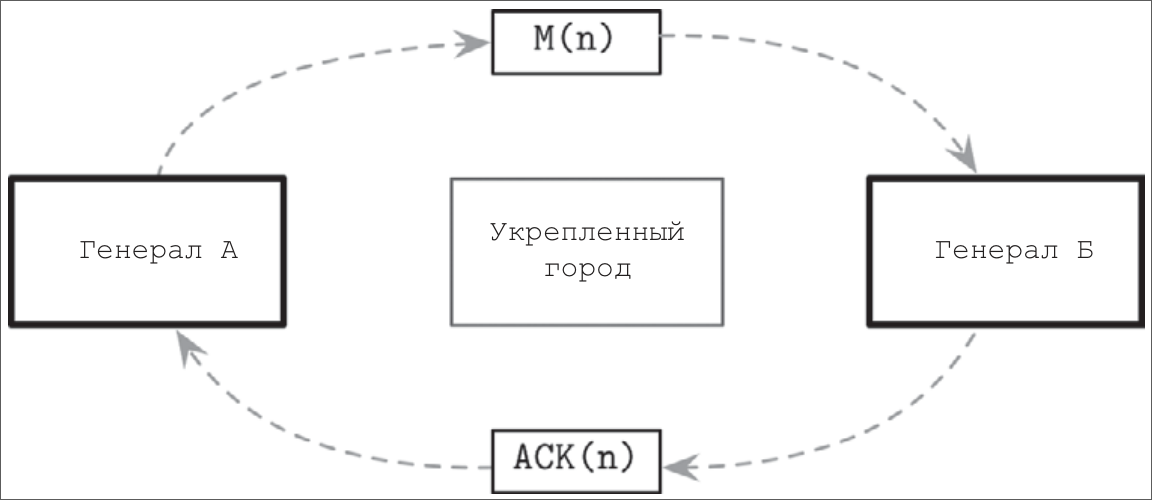
\includegraphics[scale=0.4]{inc/generals.png}
  \caption{Задача двух генералов}
  \label{fig:generals}
\end{figure}

Однако генерал А не может быть уверен, что это подтверждение дошло, оно может
быть утеряно. Чтобы устранить сомнения, требуется второе подтверждение —
ACK(ACK(MSG(N))). Этот процесс может продолжаться бесконечно, поскольку всегда
остается риск того, что последнее сообщение не достигло адресата.

В задаче не сделано предположений о времени, не установлено лимита, за которое
генералы должны ответить, связь полностью асинхронна.

В работе Фишера, Линча и Патерсона рассматривается проблема, известная как
невозможность ФЛП (FLP Impossibility) \cite{fischer85}. Эта теорема, также
именуемая теоремой Фишера–Линча–Патерсона, изучает консенсус в системах, где
процессы начинают с начального значения и стремятся согласовать новое общее
значение. После выполнения алгоритма это значение должно быть одинаковым для
всех корректно работающих процессов.

В исследовании предполагается полностью асинхронная среда, где процессы не
имеют общего времени. Алгоритмы в таких системах не могут полагаться
на время ожидания, а у процесса отсутствует возможность определить, отказал ли
другой процесс или просто работает медленно. В статье доказывается, что при
указанных предположениях невозможно создать протокол, который гарантирует
достижение консенсуса за ограниченное время. Даже один сбой процесса, не
сопровождающийся уведомлением, делает консенсус недостижимым для полностью
асинхронной распределенной системы.

Тем не менее, теорема ФЛП не утверждает, что достижение консенсуса в принципе
невозможно. Она лишь показывает, что в асинхронной системе консенсус не всегда
достижим за конечное время. В реальных системах часто присутствует некоторая
степень синхронности, и эту особенность нужно учитывать.

\subsection{Синхронность}

Из теоремы ФЛП следует, что ключевой характеристикой распределенной системы
является предположение о времени. В асинхронных системах невозможно
гарантировать ограниченные задержки в доставке сообщений, упорядоченность их
получения. Процесс выдает ответ через неопределенной долгое время.

Однако, одним из аргументов против асинхронных систем является их оторванность
от реальности: процессы не имеют произвольно разные скорости обработки, а
задержки передачи сообщений не бывают бесконечными.

Можно сделать предположения менее строгими, считая систему синхронной. Может
предполагаться, что процессы работают с сопоставимыми скоростями, задержки
передачи сообщений в канале ограничены, их доставка не может занимать
бесконечно долгое время.

В модель синхронной системы также можно добавить локальные для процесса
синхронизированные часы: при этом существует некоторая верхняя граница в раз­
нице во времени между двумя локальными для процессов источниками времени
\cite{cachin11}.

Свойства асинхронных и синхронных моделей можно объединить, рассматривая
систему как частично синхронную. Частично синхронная система обладает некото­
рыми свойствами синхронной системы, но при этом ограничения на время доставки
сообщений, уход показаний часов и относительные скорости обработки могут быть
приблизительными и действовать лишь в большинстве случаев.

\subsection{Модели отказов}

Модель отказов описывает, каким образом могут происходить сбои в работе
процессов распределенной системы. Например, можно предположить, что процесс
может полностью завершить работу и не восстановиться, восстановиться через
некоторое время или начать выдавать некорректные данные из-за сбоя или
преднамеренно.

Поскольку процессы в распределенных системах взаимодействуют друг с другом
при выполнении алгоритма, сбои в одном из них могут нарушить выполнение всей
системы. Для разработки алгоритмов в распределенных системах необходимо понимать,
какие отказы могут случиться, чтобы правильно обрабатывать каждый из них.

\subsubsection*{Аварийное завершение}

В этой модели предполагается, что процесс перестает выполнять шаги алгоритма
и не отправляет сообщений другим процессам. После сбоя процесс остается в этом
состоянии и больше не участвует в текущем выполнении алгоритма.

Важно отметить, что эта модель не запрещает восстановление процессов. Процесс
может восстановиться, синхронизироваться с текущим состоянием системы и
участвовать в новых раундах алгоритма.

Процесс, который восстанавливается после сбоя, может продолжить выполнение с
последнего известного ему шага. Алгоритмы, поддерживающие восстановление,
должны вводить в систему понятия устойчивого состояния алгоритма и протокола
восстановления \cite{skeen83}.

\subsubsection*{Пропуск}

В этой модели процесс пропускает выполнение отдельных шагов алгоритма, либо
эти шаги невидимы для других участников, либо процесс не может отправлять и
получать сообщения. Пропуски включают сетевые сбои, вызванные неисправностями
каналов связи, отказами оборудования или перегрузкой сети.

Пропуски возникают, когда алгоритм не завершает определенные действия, или их
результаты не достигают других процессов. Например, потерянное сообщение может
привести к тому, что отправитель считает его доставленным, несмотря на его
окончательную утрату.

\subsubsection*{Византийские ошибки}

Произвольные, или византийские, ошибки (Byzantine faults) представляют собой
наиболее сложный класс отказов. В этом случае процесс продолжает выполнять шаги
алгоритма, но делает это некорректно.

Такие сбои могут быть вызваны ошибками в программном обеспечении, выполнением
разных версий алгоритма или намеренными действиями злоумышленников. Например,
в распределенных системах без централизованного управления, таких как
криптовалюты, процессы могут фальсифицировать данные, чтобы ввести систему в
заблуждение.

\subsubsection*{Обработка отказов}

Одним из способом обработки отказов при невизантийских ошибках является введение
в алгоритм избыточности. Таким образом отказ может быть замаскирован: даже если
один или несколько процессов откажут, то пользователь этого не заметит
\cite{christian91}. Raft и Paxos, которые будут рассмотрены в данной работе,
основываются на модели отказов и минимизирует влияение отказов путем
использования избыточности процессов.

В случае работы в распределенной системе с византийскими ошибками используется
перекрестная проверка других узлов на каждом шаге, поскольку узлы не могут
полагаться друг на друга или на лидера и должны проверять поведение других узлов,
сравнивая возвращаемые результаты с ответами большинства. PBFT, PoW, PoS борются
с ошибками именно так.

\subsection{Итоги}

Таким образом, к распределенной системе, в которой будет исполняться любой из
описанных в данной работе алгоритм консенсуса, применяются следующие ограничения:

\begin{itemize}
    \item Система передает сообщения по совершенным каналам, однако допустимо
        разделение сети.
    \item Необходимо учитывать возможность отказа узлов: аварийное завершение и
        пропуск части алгоритма процессом.
    \item В системе невозможны византийские ошибки. Предполагается, что все узлы
        честные и выполняют свои функции корректно.
    \item Система является частично синхронной, в ней существует понятие времени,
        которое используется для синхронизации локальных часов. Сообщения в системе
        могут отправляться бесконечно, процессы могут работать с произвольной
        скоростью.
\end{itemize}

    \section{Paxos}

Алгоритм Паксос (Paxos) считается одним из самых известных методов достижения
консенсуса. Его предложил Лесли Лэмпорт в своей работе The Part-Time
Parliament («Парламент с неполной занятостью») \cite{lamport98}. В данной
статье идея консенсуса была представлена через метафору законодательного
процесса и голосования, происходящих на острове Паксос. Позднее, в 2001 году,
Лэмпорт опубликовал статью Paxos Made Simple («Простой Паксос») \cite{lamport01},
где использовал упрощенную терминологию, которая и используется в данной работе.

В рамках алгоритма Паксос участники могут выполнять одну из трех ролей:

\begin{itemize}
    \item Заявители (proposers). Принимают значения от клиентов, формируют
        предложения для их утверждения и пытаются получить голоса акцепторов.
    \item Акцепторы (acceptors). Участвуют в голосовании за принятие или
        отклонение предложений, сформированных заявителями. Для устойчивости
        к отказам система включает несколько акцепторов, однако для принятия
        решения достаточно кворума (то есть большинства голосов).
    \item Ученики (learners). Отвечают за хранение результатов принятых решений,
        выполняя роль реплик.
\end{itemize}

В большинстве реализаций эти роли совмещены в одном процессе.

Каждое предложение содержит уникальный номер, который монотонно увеличивается,
и значение, предложенное клиентом. Номер предложения используется для установления
общего порядка операций и определения их последовательности («до» или «после»).
Номера предложений часто оформляются как пара (идентификатор узла и временная метка).
Идентификаторы узлов являются упорядочиваемыми и могут быть использованы для
разрешения конфликтов между временными метками. Для корректной работы алгоритма
требуется синхронизация локальных часов.

\subsection{Алгоритм Paxos}

Алгоритм Паксос можно разделить на два ключевых этапа: голосование (или этап
предложения) и репликацию. На этапе голосования заявители борются за установление
своего лидерства, а на этапе репликации заявитель распространяет согласованное
значение среди акцепторов.

Заявитель выступает как начальная точка контакта для клиента, получая значение,
которое должно быть принято, и пытается собрать голоса от акцепторов. После
этого акцепторы рассылают информацию о принятом значении среди учеников, что
позволяет ответить пользователю. Ученики, в свою очередь, увеличивают
коэффициент репликации согласованного значения.

Только один заявитель может получить большинство голосов. В случае, если
голоса распределяются равномерно, ни один из заявителей не сможет набрать
большинство, и тогда им придется начать процесс заново.

На этапе предложения заявитель отправляет запрос $Подготовка(n)$ (где $n$ —
номер предложения) большинству акцепторов, пытаясь собрать их голоса. Акцептор,
получив запрос, должен ответить, соблюдая несколько инвариантов \cite{lamport01}:

\begin{itemize}
    \item Если акцептор еще не отвечал на запрос с более высоким порядковым
        номером, он обещает не принимать предложения с меньшими номерами.
    \item Если акцептор уже принял какое-то предложение, он уведомляет
        заявителя о принятом значении через сообщение $Обещание(m, vпринятых)$.
    Если акцептор ранее ответил на запрос с большим порядковым номером, он уведомляет заявителя о существующем предложении с более высоким номером.
    Акцептор может ответить на несколько запросов, если последний имеет наибольший порядковый номер.
\end{itemize}

Когда заявитель получает большинство голосов, начинается этап репликации. Заявитель фиксирует предложение, отправляя акцепторам сообщение Принятие(n, v), где v — это значение, соответствующее предложению с наибольшим номером среди полученных ответов от акцепторов, или собственное значение заявителя, если акцепторы не приняли других предложений.

Акцептор примет предложение с номером n, если на этапе предложения он не ответил на запрос с большим номером. Если акцептор отклоняет предложение, он отправляет заявителю максимальный порядковый номер, который он видел, для актуализации данных заявителя [LAMPORT01].

После того как консенсус относительно значения достигнут (хотя бы один акцептор принял решение), последующие заявители должны принять это значение, чтобы сохранить согласованность. Поэтому акцепторы возвращают последнее принятое значение. Если ни один акцептор не видел предыдущего значения, заявителю разрешается выбрать собственное.

Ученики получают информацию о принятом значении, когда большинство акцепторов сообщает им об этом. Акцепторы могут сразу уведомить учеников о принятом значении. При наличии нескольких учеников акцепторы должны уведомить каждого, однако можно выделить несколько учеников, которые будут отвечать за уведомление других.

Таким образом, основной целью первого этапа алгоритма является установление лидера и определение принятого значения, что позволяет перейти ко второму этапу — распространению значения. В базовом алгоритме оба этапа выполняются каждый раз, когда необходимо принять решение. Однако на практике можно уменьшить количество шагов, разрешив заявителю предложить несколько значений одновременно. Этот подход будет рассмотрен позже в разделе "Мульти-Паксос".

\subsection{Сценарии отказа}
\subsection{MultiPaxos}

    \section{Raft}

\subsection{Роль лидера в Raft}
\subsection{Добавление процессов в Raft}
\subsection{Сценарии отказа}

    \include{contents/2-04-comparison.tex}
    \section{Реализация алгоритма Raft на TLA+}

Описание TLA+.

\subsection{Формальная спецификация алгоритма}
\subsection{Проверка модели}


    \conclusion

Таким образом, в ходе прохождения практики был разработан новый протокол подключения анонимных реплик, удовлетворяющий требованиям команды CDC. Он выглядит следующим образом:

\begin{enumerate}
    \item Анонимая реплика отправляет IPROTO\_FETCH\_SNAPSHOT, сообщая мастеру, что она хочет реплицироваться с него. В этот запрос может быть включены следующие опции:
    \begin{enumerate}
        \item IPROTO\_CURSOR - реплика хочет использовать файловый JOIN для возможности продолжения подключения в случае разрыва подключения.
        \item IPROTO\_IS\_PERSISTENT\_GC - необходимо создать анонимного GC consumer и сохранять xlog файлы для данной реплики.
        \item IPROTO\_SPACE\_NAME\_FILTER - поток репликации должен быть фильтрованным. Требуются только частичные данные.
    \end{enumerate}
    \item В ответ мастер посылает vclock read-view или файла снапшота (в зависимости от IPROTO\_CURSOR). Мастер создает анонимный GC consumer, если опция IPROTO\_IS\_PERSISTENT\_GC равен true.
    \item Мастер начинает пересылку данных. Если IPROTO\_SPACE\_NAME\_FILTER указан, то данные фильтруются на стороне сервера и посылаются частично.
    \item Реплика посылает IPROTO\_SUBSCRIBE, указывая необходимость GC consumer и фильтрации потока.
\end{enumerate}

В любой момент времени процесс подключения может быть разорван и продолжен с того же момента. Ошибки удаления файлов xlog больше не возникают, так как теперь есть возможность их сохранения для анонимных реплик. Нагрузка на CDC реплики была снижена, так как теперь им больше не приходится самостоятельно обрабатывать фильтрацию репликации.


    \printbibliography

    \appendix
    \appendixsection{Спецификация Raft на TLA+}

    \appendixsection{Конфигурация модели для спецификация Raft}


\end{document}
